\clearpage
\subsubsection{Post-Test Loop} % (fold)
\label{sub:post_test_loop}

The Post-Test Loop is a looping statement that allows code to be run 1 or times. The post-test loop places the condition after the body of the loop. This means that the first time through the body of the loop must execute before the condition is checked. When it gets to the end of the body, the loop's condition is checked and the computer either jumps back to the start of the loop to repeat the body, or the loop ends and control flows on to the next statement in the code.

There are two common variants for the post-test loop: \texttt{\textbf{do...while}} and \texttt{\textbf{repeat...until}}. These work in the same way, in that they test the condition after the loop body, but the conditions they use will be different. The \textbf{\texttt{do...while}} loop repeats the body of the loop when its condition is \textbf{true}, \textbf{\texttt{repeat...until}} repeats the body of the loop when its condition is \textbf{false}. When implementing a post-test loop you must make sure that the condition you use matches the kind of loop supported by your language.

\begin{figure}[h]
   \centering
   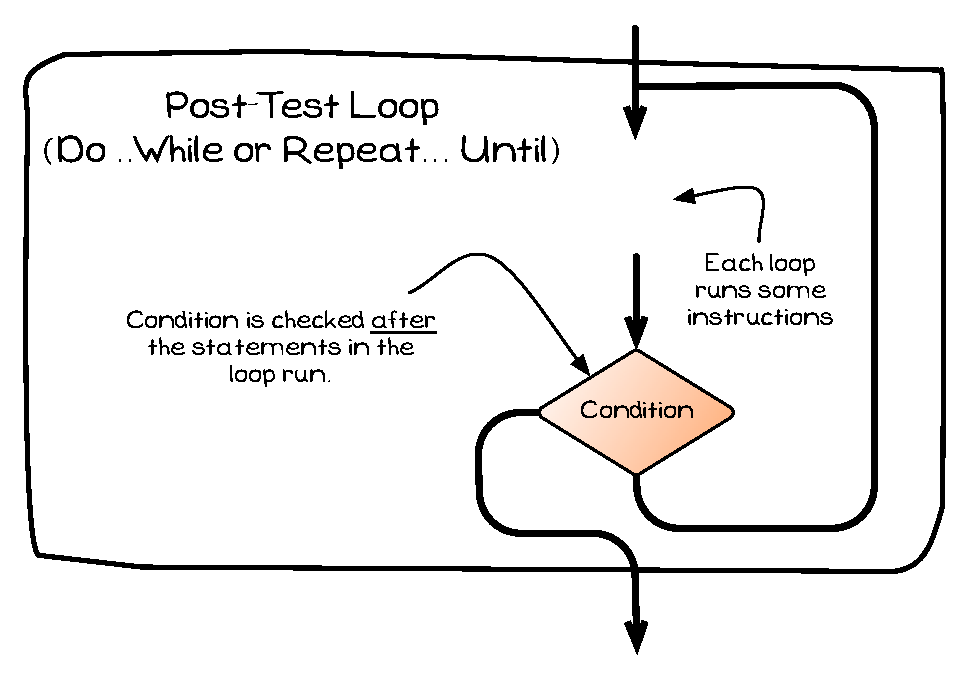
\includegraphics[width=0.9\textwidth]{./topics/control-flow/diagrams/PostTestLoop} 
   \caption{The Post-Test Loop runs the loops body, then checks the condition}
   \label{fig:looping-post-test}
\end{figure}

\mynote{
\begin{itemize}
  \item A post-test loop is an \textbf{action}, creating a loop in the code's sequence of instructions.
  \item A post-test loop allows instructions to be run 1 or more times.
  \item The condition is checked after the loop's body is executed, with control jumping back to the start if needed.
\end{itemize}
}

\csection{C includes support for the \textbf{\texttt{do...while}} loop.}
\passection{Pascal includes support for the \textbf{\texttt{repeat...until}} loop.}

% subsection post_test_loop (end)